\section{System-level Design}

\subsection{Testbench Architecture}
The design of the verification system is the major engineering challenge of this project.
% REVISIT: this sentence should be moved to intro for overall motivation of project.
While there have been many similar performance analyses done on hybrid SoCs before, each of them used their own, usually ad hoc, testbench design~\cite{Shi1}~\cite{Li1}.
As such, most testbench are not designed to be scalable or portable, serving only what they are built for.
In this project, I shall use a generic structure inspired by that of an agent in Universal Verification Methodology (UVM).

Before UVM, integrated circuit designs were verified with methodologies developed independently by stimulator vendors such as Cadence, Mentor Graphics, and Synopsys.
In an effort to unify for greater efficiency, the standards organisation of the Electronic Design Automation (EDA) industry, Accellera, established UVM with support from multiple vendors.
It provided a common structure for verification, with class libraries that made building and running a testbench a significantly smoother experience.
The agent is a container in UVM that emulates and verifies DUTs~\cite{Accellera1}.
While this project is in no position to achieve what UVM has done, I do hope that this testbench would have an easily modifiable structure that will make the process of testing similar future designs slightly simpler.

\begin{figure}[H]
  \centering
  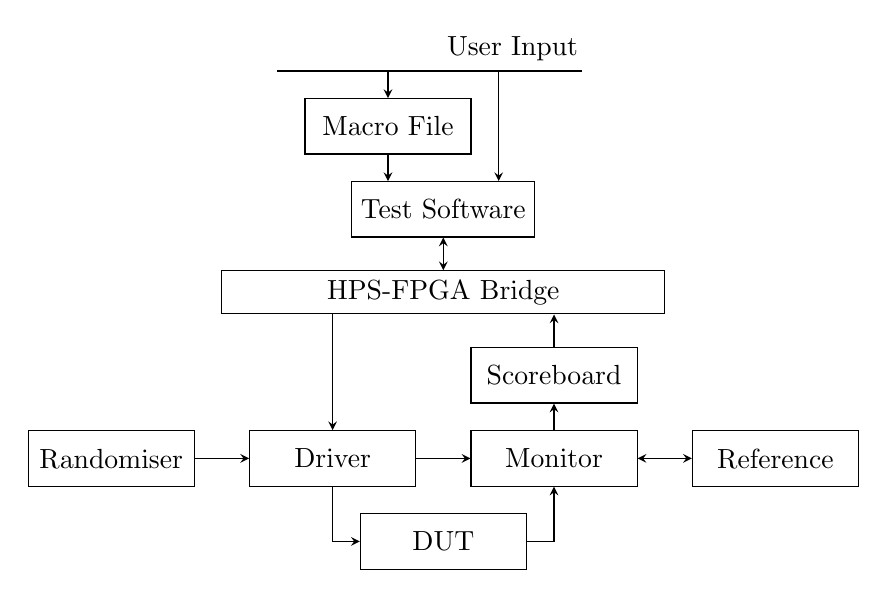
\begin{tikzpicture}
  [
    x=1em, y=1em,
    block/.style =
      {draw, rectangle, align=center, minimum width=6em, minimum height=2em},
    inter/.style =
      {draw, rectangle, align=center, minimum width=16em, minimum height=1em}
  ]
  \node [block] at (-8,3)  (r) {Randomiser};
  \node [block] at ( 0,3)  (d) {Driver};
  \node [block] at ( 4,0)  (t) {DUT};
  \node [block] at ( 8,6)  (s) {Scoreboard};
  \node [block] at ( 8,3)  (m) {Monitor};
  \node [block] at (16,3)  (u) {Reference};
  \node [inter] at ( 4,9)  (b) {HPS-FPGA Bridge};
  \node [block] at ( 4,12) (w) {Test Software};
  \node [block] at ( 2,15) (f) {Macro File};

  \draw[ ->, >=stealth] (r.east)           -- (d.west);
  \draw[ ->, >=stealth] (d.south)          |- (t.west);
  \draw[ ->, >=stealth] (t.east)           -| (m.south);
  \draw[ ->, >=stealth] (m.north)          -- (s.south);
  \draw[ ->, >=stealth] (b.south-|d.north) -- (d.north);
  \draw[ ->, >=stealth] (s.north)          -- (b.south-|s.north);
  \draw[<->, >=stealth] (b.north)          -- (w.south);
  \draw[ ->, >=stealth] (f.south)          -- (w.north-|f.north);
  \draw[ ->, >=stealth] (d.east)           -- (m.west);
  \draw[<->, >=stealth] (m.east)           -- (u.west);
  \draw[ ->, >=stealth] (2, 17)            -- (f.north);
  \draw[ ->, >=stealth] (6, 17)            -- (w.north-|6,17);

  \draw (-2,17) -- ++(6,0) -- node[above] {User Input} ++(5,0);
\end{tikzpicture}
  \caption{Block diagram of the testbench design}
  \label{Block}
\end{figure}

The test script running on the HPS will read from a configuration file, and sends the corresponding test configuration to the driver.
The driver then pulls a stream of random data generated by the randomiser, and convert them to meaningful test inputs according to specification.
The test output will be watched by the monitor, reporting any interesting event to the scoreboard, which keeps track of them.
Sub-monitors contain reference designs functionally identical to the DUT, which the monitor uses to identify false outputs from the DUT.
Multiple sub-monitors allow parallel processing, so that the reference design can have a relaxed frequency requirement.
The scoreboard tallies the events and writes them to memory locations accessible from the other side of the bridge.
These memory locations are read by the test scripts, providing results and other useful information to the user.

\subsection{User Interface}

For this evaluation framework to be meaningful, it has to attract users by being easy to configure and run.
To achieve this, 
% REVISIT: easy change of parameter in qsys, configuration file interface, maybe someof this is more like inplementation
